\chapter{Kerr black holes with self-interacting scalar hair}
\label{ch:SI}

\epigraph{``\emph{
Það man hún fólkvíg \\
fyrst í heimi, \\
er Gullveigu \\
geirum studdu \\
og í höll Hárs \\
hana brenndu, \\
þrisvar brenndu, \\
þrisvar borna, \\
oft, ósjaldan; \\
þó hún enn lifir. 
} 
''}{21st verse of Völuspá}


%%%%%%%%%%%%%%%%%%%%%%%%%%%%%%%%%%%%%%%%%%%%%%%%%%%%%%%%%%%%%%%%%%%%%%%%%%%%%%%
\section{Introduction}
% %%%%%%%%%%%%%%%%%%%%%%%%%%%%%%%%%%%%%%%%%%%%%%%%%%%%%%%%%%%%%%%%%%%%%%%%%%%%%%%
Boson stars are self-gravitating solitons.
In their simplest guise, they arise as solutions of General Relativity minimally coupled to a massive, free, complex scalar field\cite{Kaup:1968zz,Ruffini:1969qy}.
This simple model presents only two dimensionful parameters (or scales): Newton's constant $G$ (which can be rephrased as the Planck mass $M_{\rm Pl}$) and the scalar field mass $\mu$.
As for fermionic stars, the scalar field effective pressure cannot withstand an infinite amount of mass without undergoing gravitational collapse into a black hole (BH).
Intuitively, the smaller the scalar field mass, the larger the maximal mass of the star can be, since the scalar particle's Compton wavelength is larger and hence these particles are less confined. 
Indeed, actual calculations show this maximal mass is of the order of the scalar field's Compton wavelength
\begin{equation}
 M_{\rm ADM}^{\rm max}\simeq \alpha_{\rm BS} \frac{M_{\rm Pl}^2}{\mu}\simeq \alpha_{\rm BS} \, 10^{-19}M_\odot\left(\frac{\rm GeV}{\mu}\right)\ , 
\label{mini}
\end{equation}
where $M_{\odot}$ is the Sun's mass and $\alpha_{\rm BS}$ is found, numerically, to be of order of unity.
Observe that the maximal mass is small, by astrophysics standards, for scalar field masses within the range of the standard model of particle physics.
As such, these boson stars are usually called \textit{mini-}boson stars\cite{Schunck:2003kk} in the literature. 

The scalar field profile of such a boson star generally has a number of nodes, or roots, $n\in \mathbb{N}_0$. The $n=0$ case corresponds to fundamental states whereas $n>0$ are excited states. We shall focus on the former, since they are the most stable configurations.
Furthermore, we will study solutions with $m=1$, where $m$ is the azimuthal harmonic index.
It has been shown that the maximal mass increases with increasing $m$.\cite{Liebling:2012fv,Yoshida:1997qf,Grandclement:2014msa}
This increase, however, requires  unreasonably high values of $m$, for the mass to be of order $M_{\odot}$, when $\mu$ is in the mass range of standard model particles. Ultra-light scalar fields
, on the other hand, can yield astrophysical masses even for small $m$. 

A different approach to increase the maximal mass of boson stars is to include self-interactions for the scalar field.
It was found by Colpi et al.\cite{Colpi:1986ye} that for spherically symmetric \textit{quartic}-boson stars the maximal mass can be considerably higher:

\begin{equation}
 M_{\rm ADM}^{\rm max}\simeq 
0.062  \sqrt{\lambda}\frac{M_{\rm Pl}^3}{\mu^2}\simeq 0.062  \sqrt{\lambda}M_\odot \left(\frac{\rm GeV}{\mu}\right)^2\ .
\label{csw}
\end{equation}
Here, $\lambda>0$ is the self-interaction coupling where the self-interaction potential is given by $V(|\Psi|)=\lambda|\Psi|^4$.
It is therefore clear that by choosing a suitable $\lambda$, an astrophysically relevant mass can be obtained for boson stars, even for values of $\mu$ within typical of standard model particles.

For rotating boson stars, similar results were found by Ryan~\cite{Ryan:1996nk} for the large self-interaction limit, while later work considered a single value of the coupling and higher $m$ solutions.
~\cite{Grandclement:2014msa,Kleihaus:2015iea}
In this chapter, we will present a more systematic study of rotating quartic-boson stars in terms of $\lambda$.
In particular, the analogue of Eq.~\eqref{csw} was obtained for $m=1$ solutions ($cf.$ Fig.~2 in Ref.~\cite{Herdeiro:2015tia}):
%
\begin{equation}
M_{\rm ADM}^{\rm max}\simeq 
0.057  \sqrt{\lambda}\frac{M_{\rm Pl}^3}{\mu^2}\simeq 0.057  \sqrt{\lambda}M_\odot \left(\frac{\rm GeV}{\mu}\right)^2\ .
\label{quartic_rotating}
\end{equation}

However, our interests do not lie solely in the area of boson stars.
We want to consider black hole solutions with self-interacting scalar hair.
Therefore one may ask, what the maximal \textit{horizon} mass, rather than ADM mass, for KBHsSH is.
The former is well defined in terms of a Komar integral.
A first analysis of horizon mass and angular momentum for KBHsSH was presented in~\cite{Herdeiro:2015moa} where it was pointed out that the Kerr bound can be violated in terms of horizon quantities.

% The goal of this chapter is to make a different observation: the maximum horizon mass $M^{\rm max}_H$ for KBHsSH is attained at a particular configuration we dub the \textit{Hod point}, corresponding to the extremal (vacuum) Kerr BH obtained in the vanishing hair limit, and precisely one of the points studied in~\cite{Hod:2012px}.
% For KBHsSH this maximal mass obeys the same form as \eqref{mini},
% \begin{equation}
%   M_{\rm H}^{\rm max}\simeq \alpha_{\rm Hod} \frac{M_{\rm Pl}^2}{\mu}\simeq \alpha_{\rm Hod} \, 10^{-19}M_\odot\left(\frac{\rm GeV}{\mu}\right)\ , 
% \label{hodpoint}
% \end{equation}
%  but with the constant $\alpha_{\rm Hod}<\alpha_{\rm BS}$. For instance, for $m=1;2$, $\alpha_{\rm Hod}=0.526; 1.165$. 
 
%%%%%%%%%%%%%%%%%%%%%%%%%%%%%%%%%%%%%%%%%%%%%%%%%%%%%%%%%%%%%%%%%%%%%%%%%%%%%%%
\section{The model}
\label{SIsec_model}
%%%%%%%%%%%%%%%%%%%%%%%%%%%%%%%%%%%%%%%%%%%%%%%%%%%%%%%%%%%%%%%%%%%%%%%%%%%%%%% 
 
We shall consider a massive, complex scalar field, $\Psi$, minimally coupled to Einstein's gravity. The action is:
%
\begin{eqnarray}
  \label{Intaction}
  &&
	\mathcal{S} = \int d^4x \sqrt{-g}\left[\frac{R}{16\pi G}- g^{ab}\Psi^*_{,a}\Psi_{,b} - U(|\Psi|)\right],~~{~~} \ \  
\\
\label{pot}
&&~~~~{\rm with}~~~U(|\Psi|)= \mu^2\left|\Psi\right|^2 + \lambda\left|\Psi\right|^4,
\end{eqnarray}  
where $G$ is Newton's constant, $\mu$ is the scalar field mass and the self-coupling is positive, $ \lambda>0$. 
%
To describe both spinning boson stars and KBHsSH we take the metric and field ansatz defined by Eq. \eqref{eqn:HBH-ansatz} and \eqref{eqn:field-ansatz}.

The Einstein-Klein-Gordon equations obtained from \eqref{Intaction} yield a system of five coupled, non-linear PDEs, together with two constraint equations, found 
by taking $\mu^2\to \mu^2+ \lambda \phi^2$ ($\mu^2\to \mu^2+2\lambda \phi^2$) in the Einstein (Klein-Gordon) equations, as displayed in~\cite{Herdeiro:2015gia}.
The boundary conditions used to solve these
equations are different depending on considering boson stars or KBHsSH, but do not depend on $\lambda$, and can also be found in Appendix \ref{BCs}.


%%%%%%%%%%%%%%%%%%%%%%%%%%%%%%%%%%%%%%%%%%%%%%%%%%%%%%%%%%%%%%%%%%%%%%%%%%%%%%%
\section{Quartic-Boson Stars}
\label{sec_II}
%%%%%%%%%%%%%%%%%%%%%%%%%%%%%%%%%%%%%%%%%%%%%%%%%%%%%%%%%%%%%%%%%%%%%%%%%%%%%%% 
We start by considering quartic-boson star solutions and their dependence on the coupling $\lambda$. These solutions are  conveniently presented in an ADM mass $vs.$ scalar field frequency diagram, as shown in Fig. \ref{fig:w-vs-M-BSs}. In this type of diagram, for $\lambda=0$, it is well known that the boson star solutions form a spiraling curve (see $e.g.$~\cite{Herdeiro:2015gia}). The solutions start from vacuum ($w=\mu$), at which point they trivialize. As $w$ decreases from this value, their ADM mass increases until reaching a maximum value at $w_{\rm max}\simeq 0.775 \mu$. A minimum frequency is then reached after which the curve backbends towards a second branch. A second backbending and a third branch can be seen in  Fig. 1 of~\cite{Herdeiro:2015gia}.

\begin{figure}[h!]
  \begin{center}
    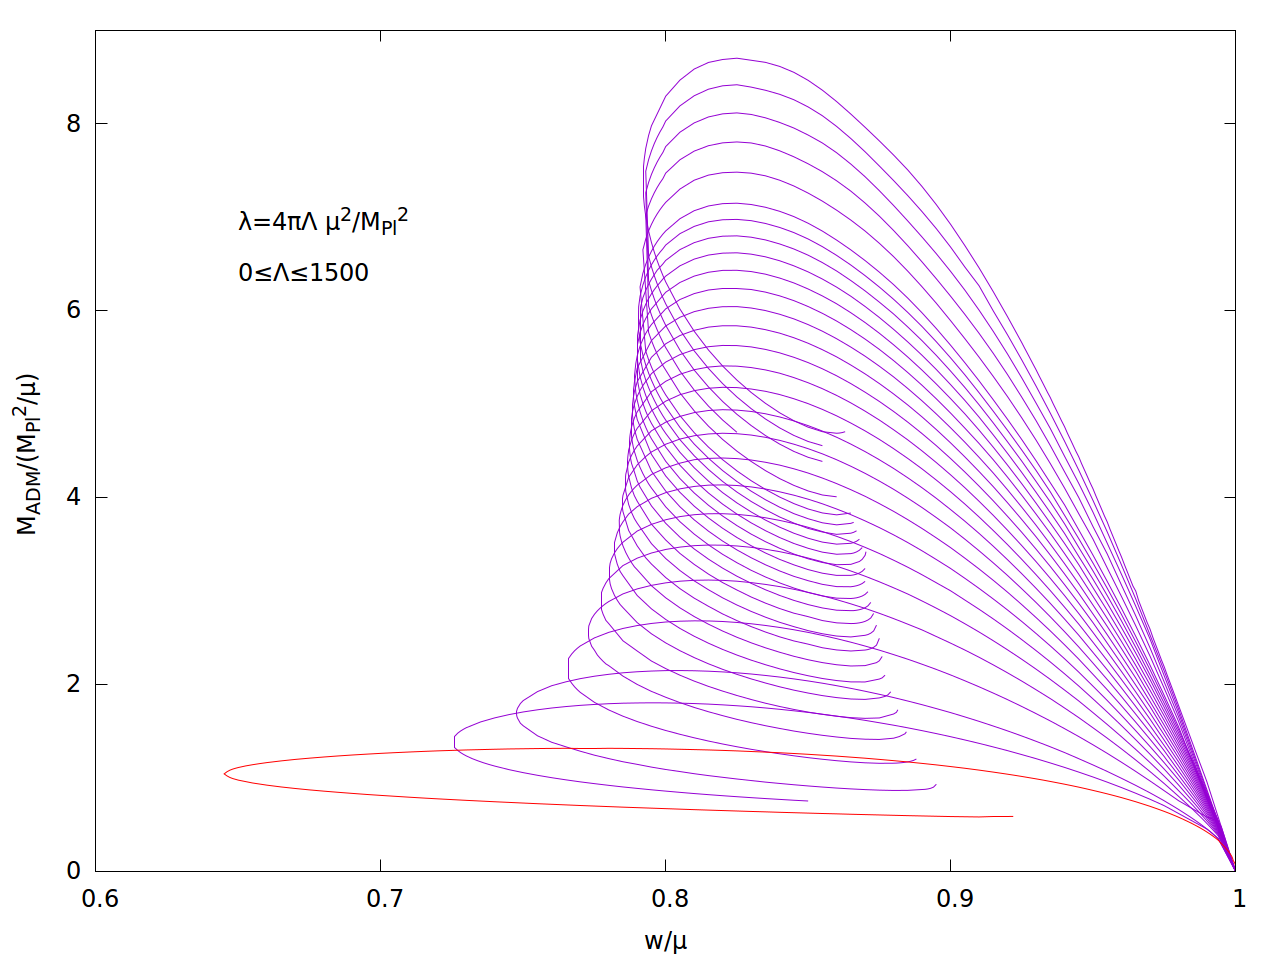
\includegraphics[width=0.7\textwidth]{papers/selfInteractions/w-vs-M-BSs2.png}
  \end{center}
  \caption{ADM mass of $m=1$, nodeless boson stars, as a function of $w$, for various values of $\lambda$ (defined by $\Lambda$, used in numerics): (from bottom to top) $\Lambda=0$ (red curve), $\Lambda=25$, $\Lambda=50-1000$ in steps of $50$, and $\Lambda=1000-1500$ in steps of $100$. Each curve was drawn from, typically, one hundred solution points.}
  \label{fig:w-vs-M-BSs}
\end{figure}



A similar description applies for $\lambda\neq 0$. In Fig. \ref{fig:w-vs-M-BSs} we can see how boson stars change as the quartic coupling parameter $\lambda$ varies from zero -- the mini-boson star case -- to a large value. The typical trend is that the spiral-like behaviour is still kept as $\lambda$ increases, with an increase of the maximal mass. Also, the range of frequencies becomes slightly smaller with increasing coupling. Each curve in Fig. \ref{fig:w-vs-M-BSs} continues after the local minimum of the mass towards a third branch which has been omitted for simplicity, but can be observed in the plots of the next section. Finally, observe that all boson star curves merge at the origin, where they trivialize. 

From the data exhibited in Fig.~\ref{fig:w-vs-M-BSs} one obtains the  maximal mass $M_{\rm ADM}^{\rm max}$ $vs.$ $\lambda$ exhibited in Fig.~\ref{max_mass_0}; for large $\lambda$ the data points are well fitted by the formula announced in the Introduction: \eqref{quartic_rotating}.
%
\begin{figure}[h!]
  \begin{center}
    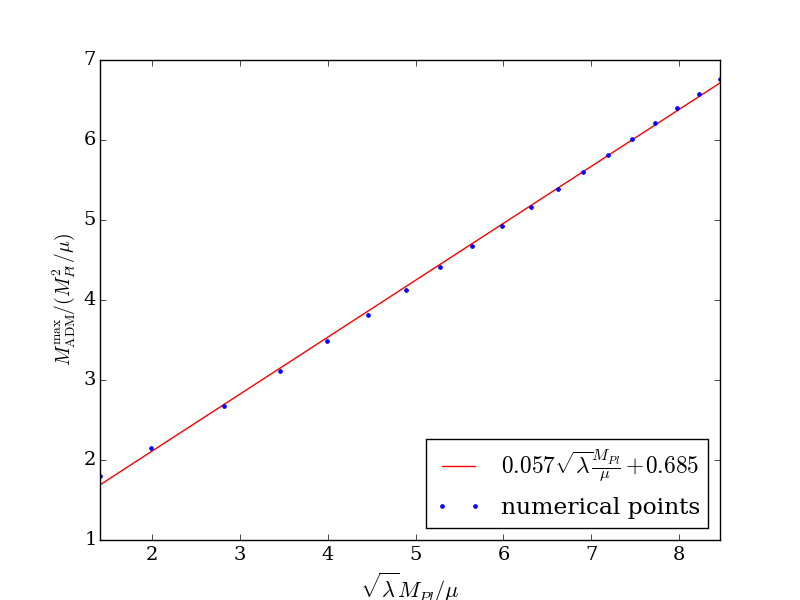
\includegraphics[width=0.7\textwidth]{papers/selfInteractions/max-mass.png}
  \end{center}
  \caption{$M_{\rm ADM}^{\rm max}$ for boson stars $vs.$ the coupling constant $\lambda$, using the data in Fig.~\ref{fig:w-vs-M-BSs}, together with a numerical fit.}
  \label{max_mass_0}
\end{figure}
%






%%%%%%%%%%%%%%%%%%%%%%%%%%%%%%%%%%%%%%%%%%%%%%%%%%%%%%%%%%%%%%%%%%%%%%%%%%%%%%%
\section{Quartic-KBHsSH: ADM quantities}
\label{sec_III}
%%%%%%%%%%%%%%%%%%%%%%%%%%%%%%%%%%%%%%%%%%%%%%%%%%%%%%%%%%%%%%%%%%%%%%%%%%%%%%%
We now turn to KBHsSH and consider first no self-interactions. For nodeless, $m=1$ KBHsSH, their domain of existence, in an ADM mass $vs.$ $w$~\cite{Herdeiro:2014goa,Herdeiro:2015gia} is shown in the left panel of Fig.~\ref{kbhsh1}.  The black solid line represents extremal BHs {with horizon angular velocity}
\begin{eqnarray}
\label{SIcond}
 \Omega_H=\frac{w}{m} \ .
\end{eqnarray} 
We recall this is the synchronization condition which underlies KBHsSH. (Vacuum) Kerr BHs exist in this diagram below this line. The domain of existence of KBHsSH is bounded by:
\begin{description}
\item[i)] the corresponding boson star curve (red solid line), for which we display the first three branches;
\item[ii)] by a line of extremal ($i.e.$ zero temperature) KBHsSH (green dashed line);
\item[iii)] and by a line of (vacuum) Kerr BHs (blue dotted line), corresponding to the Kerr solutions that allow the existence of stationary scalar clouds with the appropriate set of quantum numbers~\cite{Herdeiro:2014goa,Benone:2014ssa}.   
\end{description}
The ``Hod point" (grey dot) lies at the intersection of boundaries ${\bf ii)}$ and ${\bf iii)}$, corresponding to the extremal (vacuum) Kerr BH obtained in the limit of vanishing scalar field. Remarkably,  at the Hod point, the scalar field possesses a relatively simple closed form~\cite{Hod:2012px}.
% in terms of hypergeometric functions and spheroidal harmonics.


When a quartic self-interaction is included for the scalar field, it was already shown in~\cite{Kleihaus:2015iea} that a similar pattern occurs, for a particular value of the coupling. In the right panel of Fig.~\ref{kbhsh1} we show the domain of existence of KBHsSH for four different values of the coupling $\lambda$, given by $\Lambda=0,100,350.70$. Each domain of existence has been filled in by thousands of numerical points. As can be observed, as the coupling is varied, boundaries  ${\bf i)}$ and ${\bf ii)}$ change, and seem to be delimiting a gradually thinner ribbon in this diagram. Boundary  ${\bf iii)}$, however, is invariant, and so is the Hod point, as the self-interaction of the scalar field become irrelevant in the probe limit. In particular, this analysis confirms that the maximal ADM mass for quartic-KBHsSH is that of the corresponding boson stars, and so it is still given by~\eqref{quartic_rotating}.




\begin{figure}[h!]
  \begin{center}
    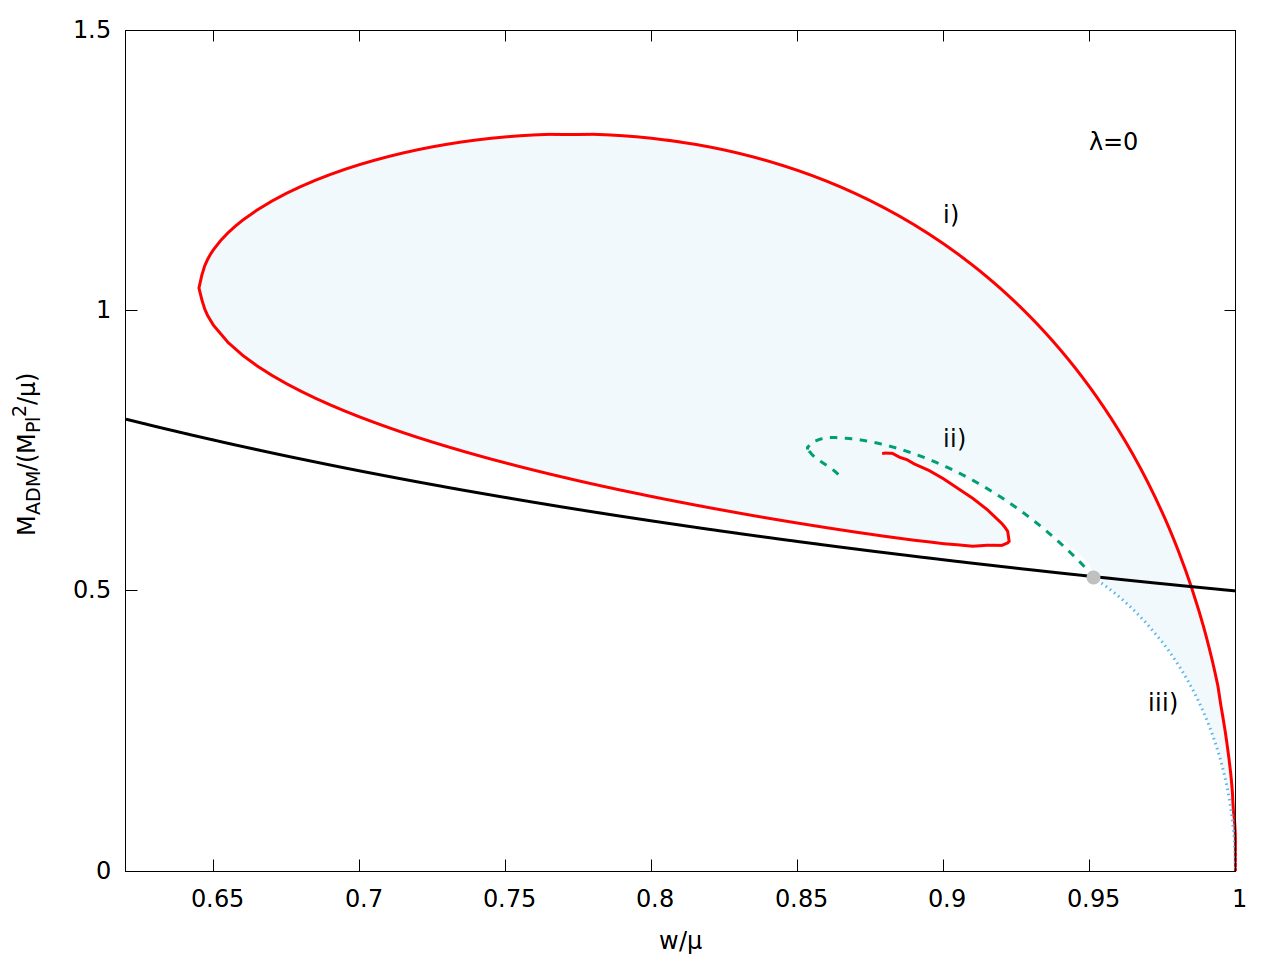
\includegraphics[width=0.48\textwidth]{papers/selfInteractions/w-vs-M-0.png}
    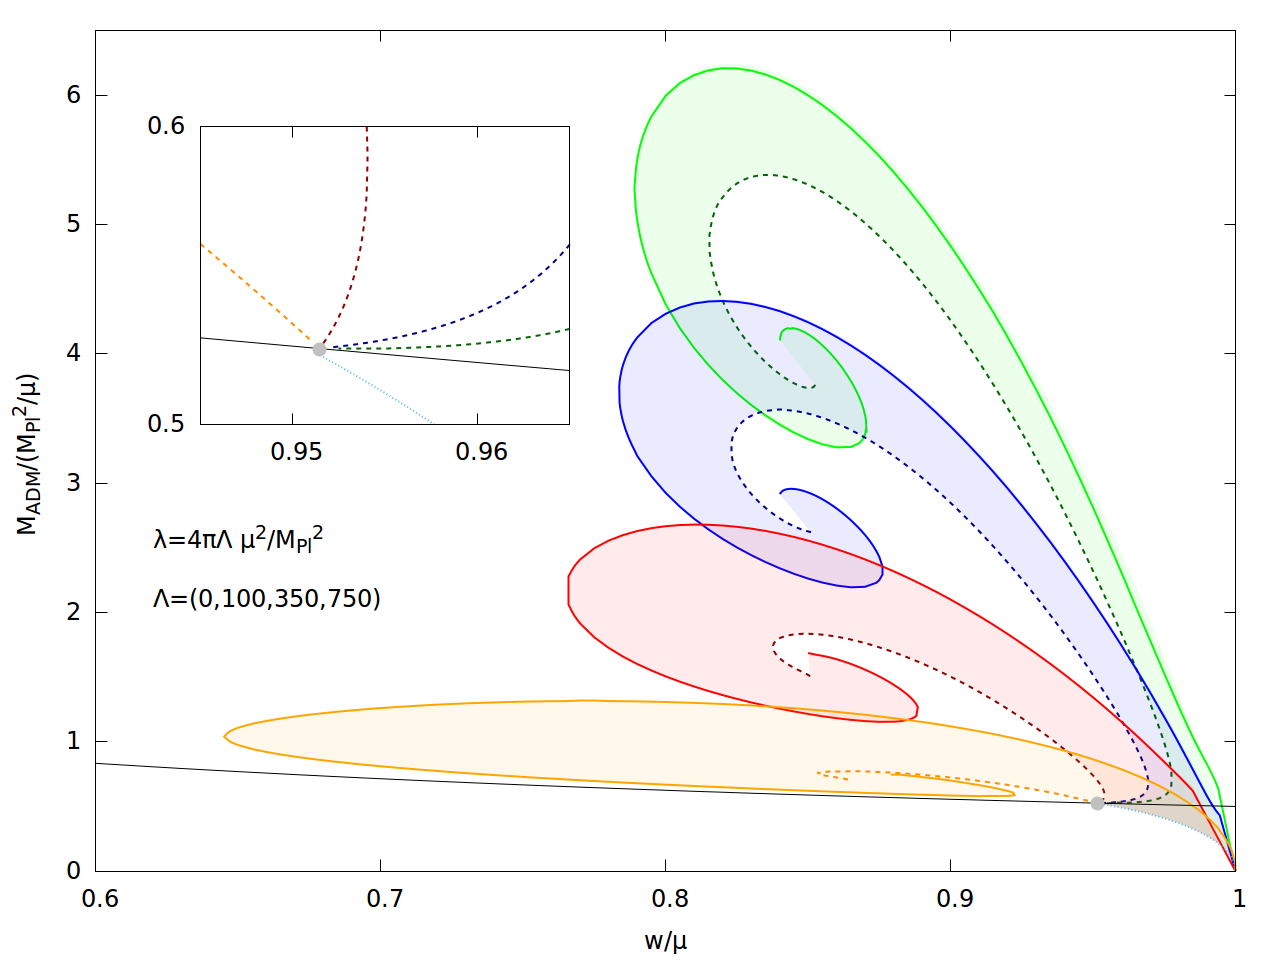
\includegraphics[width=0.48\textwidth]{papers/selfInteractions/BH-w-Mtimes4.png}
      \end{center}
  \caption{(Left) Domain of existence of KBHsSH without self-interactions (blue shaded region).(Right) Domain of existence of KBHsSH for $\Lambda=0,100,350.70$ (shaded regions, from the lowest to the highest, respectively). The inset shows a detail around the Hod point (grey dot).}
  \label{kbhsh1}
\end{figure}


In Fig.~\ref{fig:no-HBHs} we exhibit the phase space in terms of ADM quantities for quartic-KBHsSH for the four values of the coupling also used above. As before, the red solid line denotes boson stars, the black solid line marks extremal Kerr (which means that Kerr BHs, exist \textit{above} this line, in this diagram), the blue dotted line is the zero mode line and blue shaded region is where (quartic-)KBHsSH exist. Analogously to the $\lambda=0$ case, there is always a positive correlation between the ADM mass and the ADM angular momentum, $J_{ADM}$, for the self-interacting case. In fact, the diagram looks quite similar, regardless of $\lambda$, with the major difference that, as $\lambda$ increases, larger values of $M_{\rm ADM}$ and $J_{ADM}$ are allowed. Also observe that for all cases there are solutions violating the Kerr bound, in terms of ADM quantities, as noticed for KBHsSH in~\cite{Herdeiro:2014goa,Herdeiro:2015moa} and for a specific example of quartic-KBHsSH in~\cite{Kleihaus:2015iea}.



\begin{figure}[h!]
  \begin{center}
    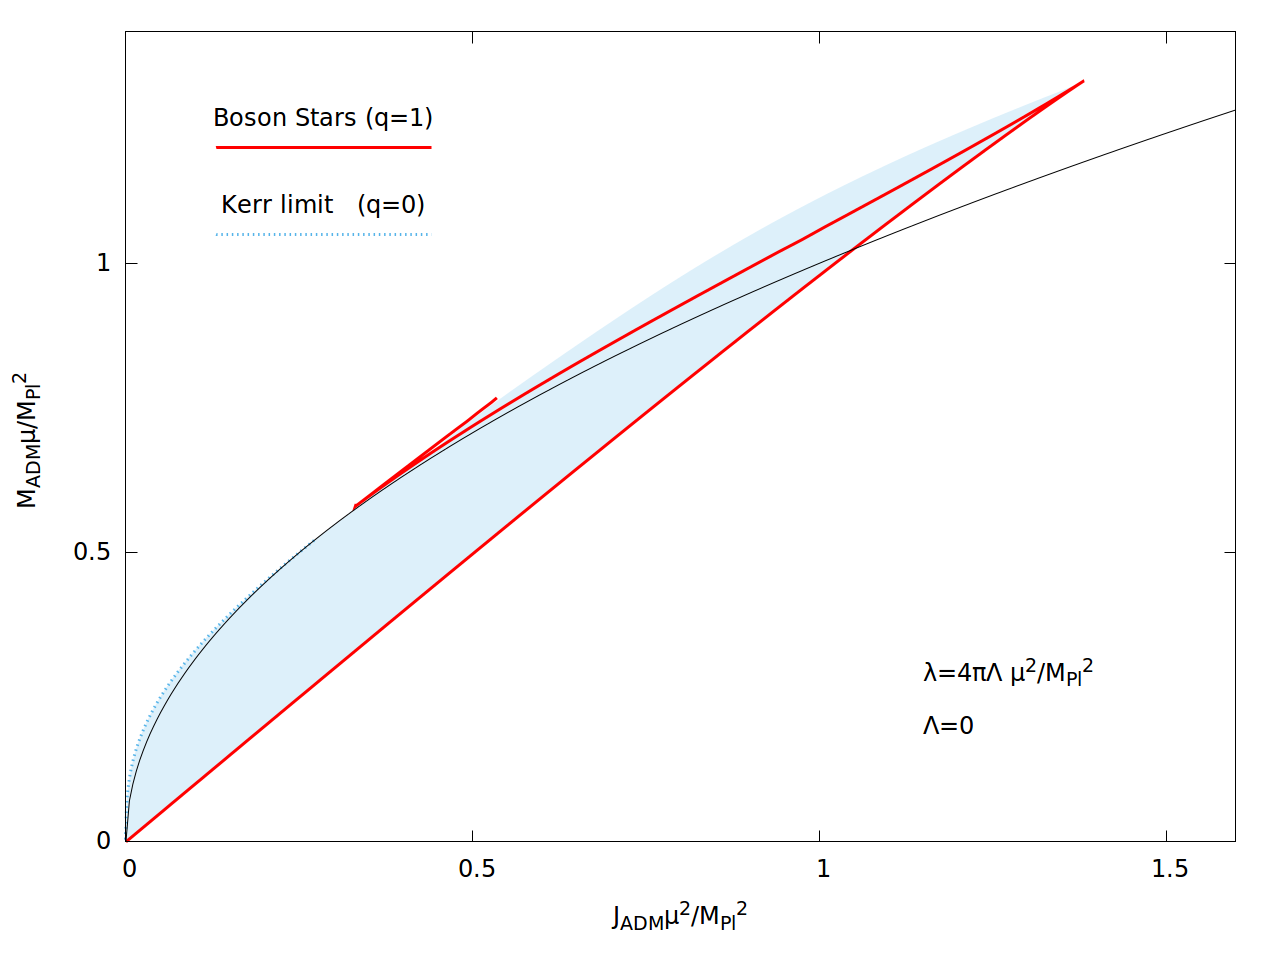
\includegraphics[width=0.48\textwidth]{papers/selfInteractions/c2=0-J-M.png}
    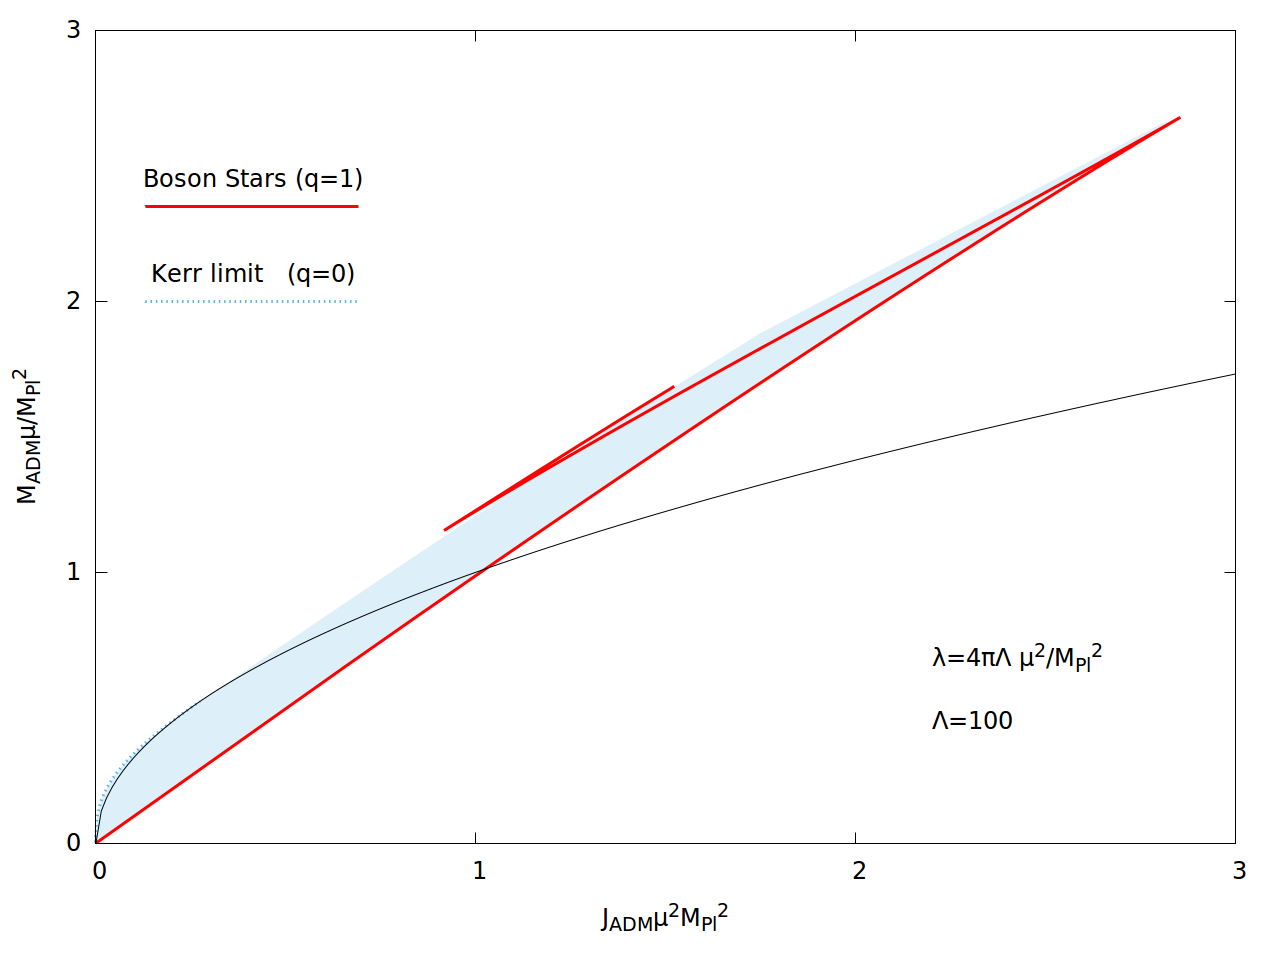
\includegraphics[width=0.48\textwidth]{papers/selfInteractions/c2=100-J-M.png}\\
    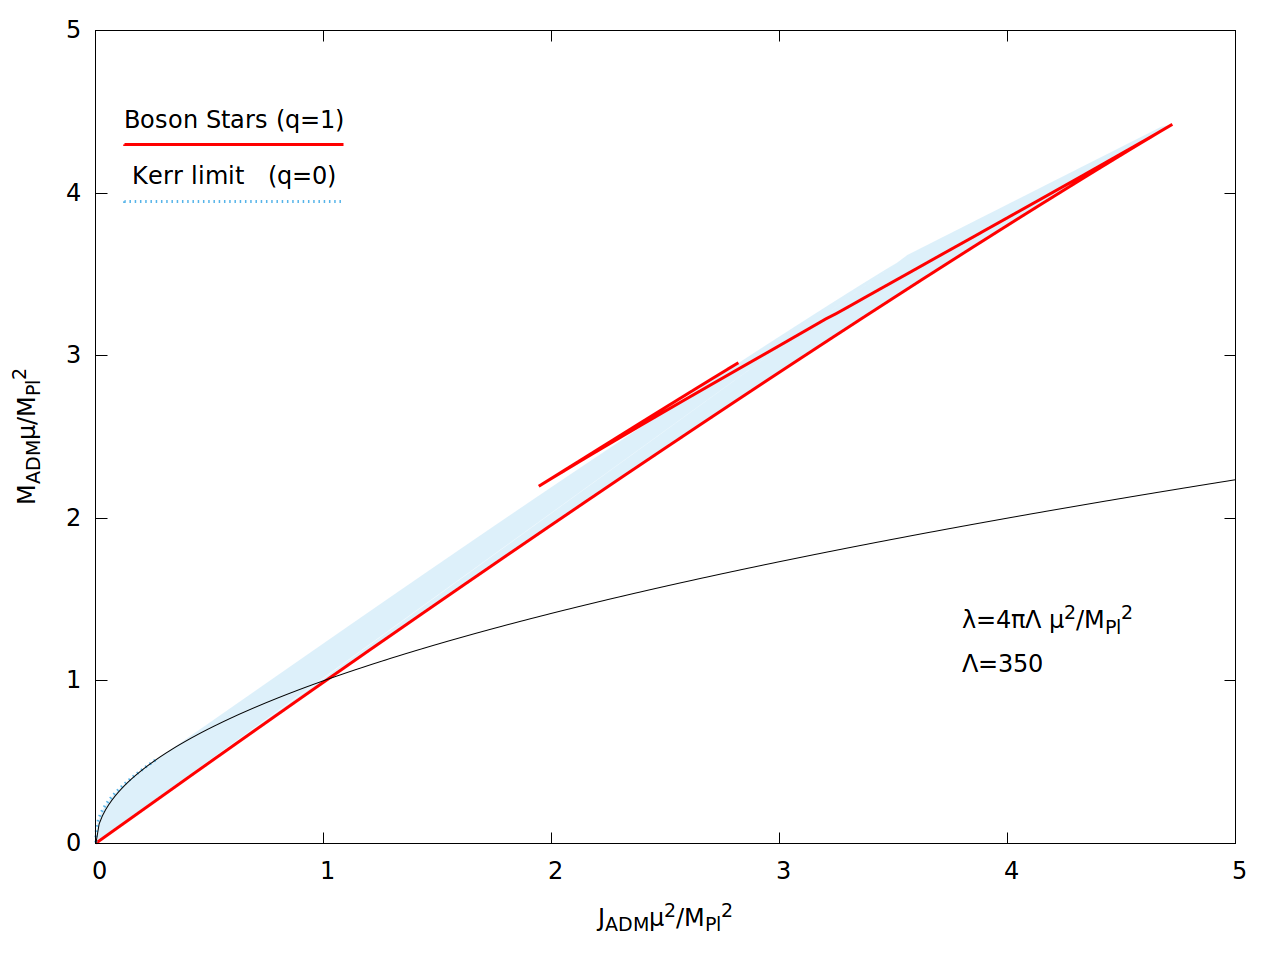
\includegraphics[width=0.48\textwidth]{papers/selfInteractions/c2=350-J-M.png}
    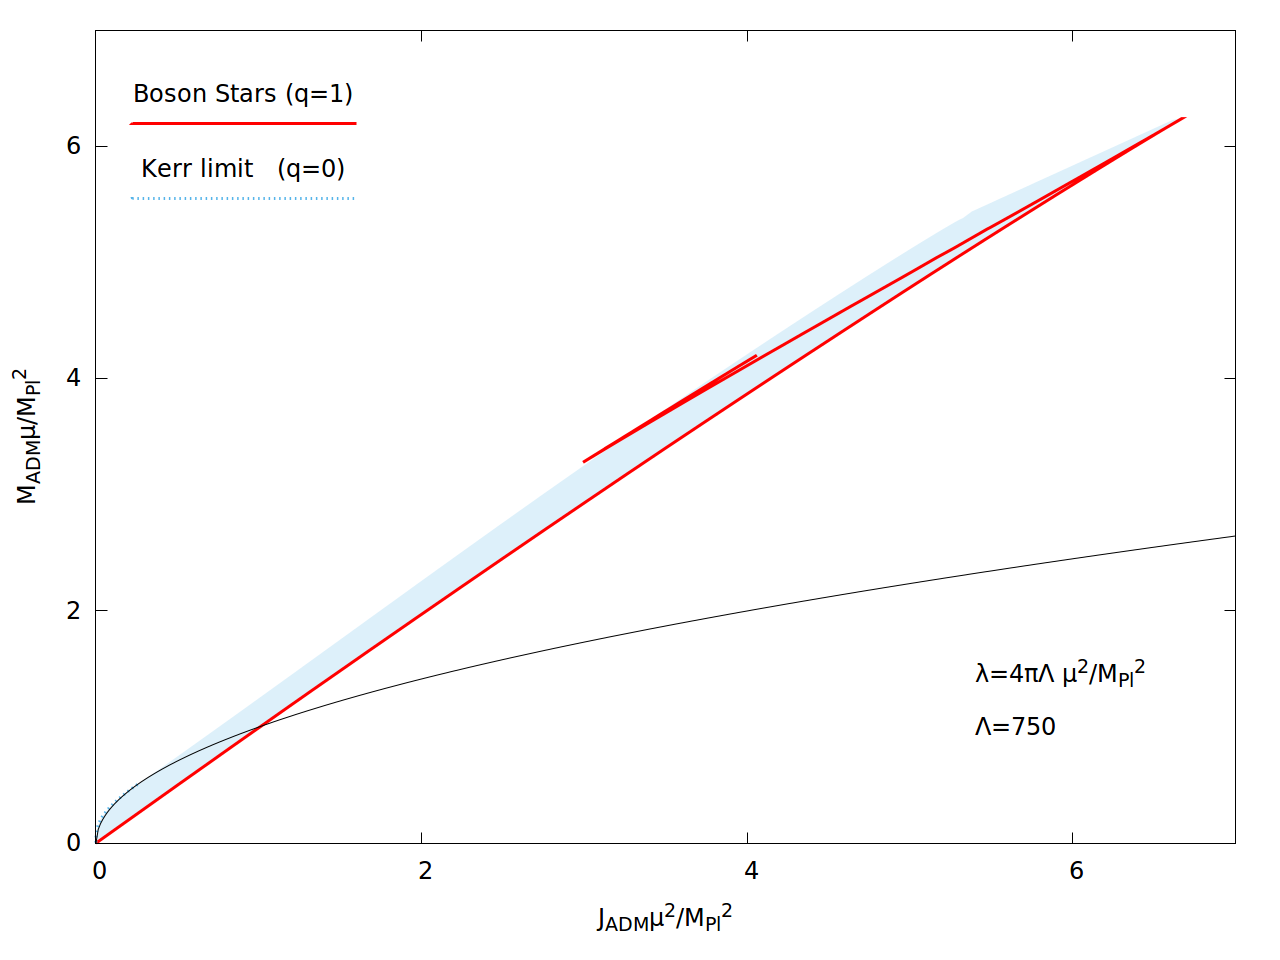
\includegraphics[width=0.48\textwidth]{papers/selfInteractions/c2=750-J-M.png}
  \end{center}
  \caption{Domain of existence of KBHsSH in an ADM mass $vs.$ ADM angular momentum diagram, for $\Lambda=0,100$ (top left and right panels) and $\Lambda=350.70$ (bottom left and right panels).}
  \label{fig:no-HBHs}
\end{figure}
 

%%%%%%%%%%%%%%%%%%%%%%%%%%%%%%%%%%%%%%%%%%%%%%%%%%%%%%%%%%%%%%%%%%%%%%%%%%%%%%%
\section{Quartic-KBHsSH: horizon quantities}
\label{sec_IV}
%%%%%%%%%%%%%%%%%%%%%%%%%%%%%%%%%%%%%%%%%%%%%%%%%%%%%%%%%%%%%%%%%%%%%%%%%%%%%%%

 
We now turn our attention to the horizon mass $M_{\rm H}$ and angular momentum $J_{\rm H}$. In Fig.~\ref{horizon_phase}, we display the phase space of quartic-KBHsSH, for a particular value of $\lambda$, but that illustrates the general pattern we have observed. 


\begin{figure}[h!]
  \begin{center}
    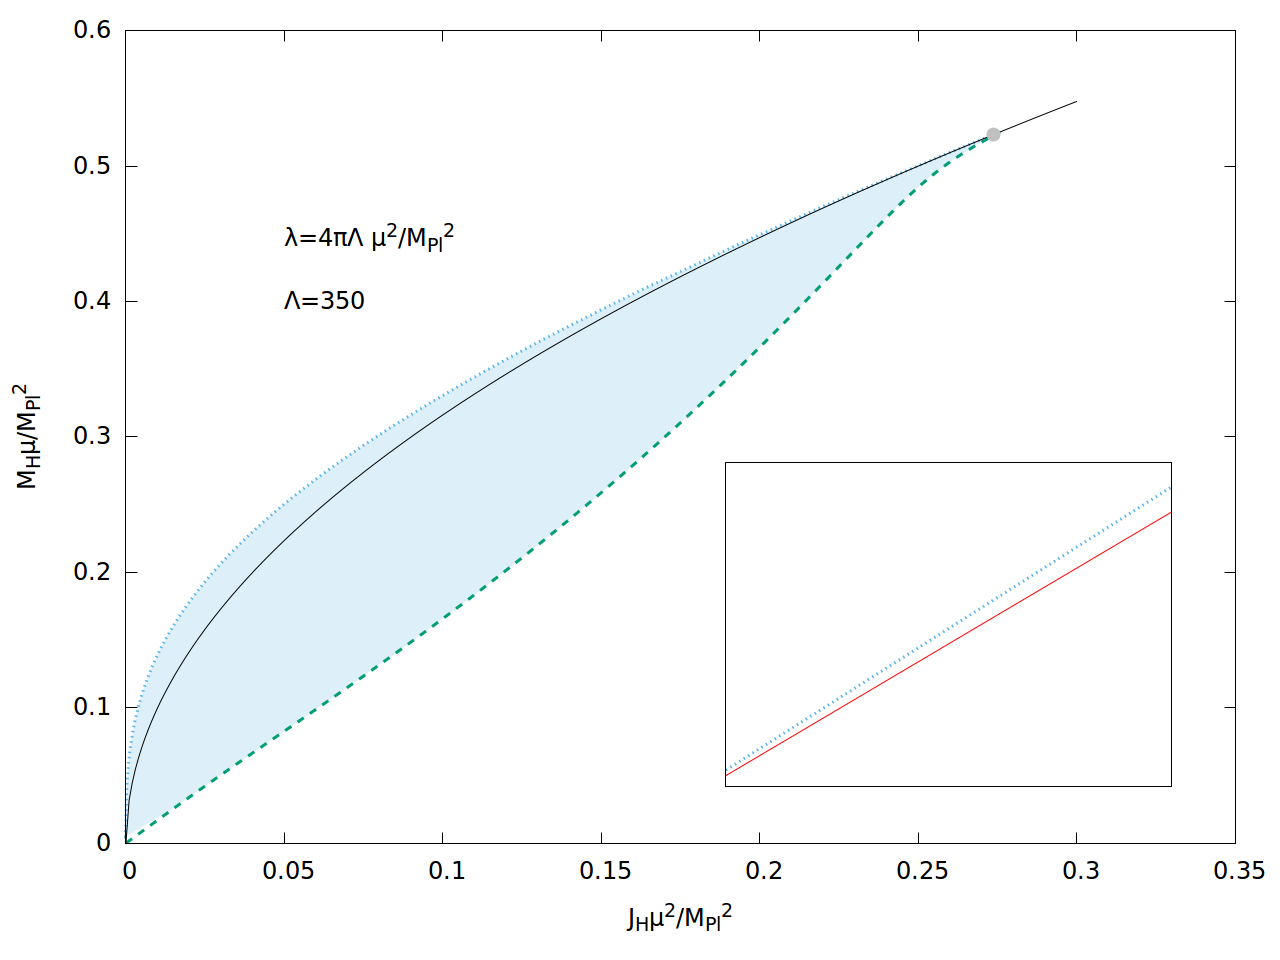
\includegraphics[width=0.7\textwidth]{papers/selfInteractions/horizon-quantities.png}
      \end{center}
  \caption{Phase space in terms of horizon quantities.}
  \label{horizon_phase}
\end{figure}

In Fig.~\ref{horizon_phase}, we can see that all solutions lie within the envelope formed by the (blue dotted) line of vacuum Kerr BHs and the (green dashed) line of extremal KBHsSH, corresponding to the blue shaded region. The salient feature we wish to emphasize is that all quartic-KBHsSH have, therefore, a \textit{lower} mass than that at the Hod point. The same pattern is observed for all other values of $\lambda$ we have studied. 


The black solid line in Fig.~\ref{horizon_phase} denotes the Kerr bound threshold, in terms of horizon quantities $J_{\rm H}=M_{\rm H}^2$ and it can be observed that there are solutions below it, thus violating the Kerr bound in terms of horizon quantities, as was observed in~\cite{Herdeiro:2015moa} for KBHsSH (without self-interactions). 

Finally, the inset of Fig.~\ref{horizon_phase} illustrates the typical pattern when starting from a given vacuum Kerr BH (on the blue dotted line) and increasing the hair, but keeping the frequency $w$ constant -- which we use as a control parameter. The corresponding points fall into the red solid line in the inset. One observes that making (vacuum) Kerr BHs hairier in this way, their horizon quantities increase, but the horizon mass increases more slowly in term of the horizon angular momentum than along the vacuum Kerr line. 


Fig.~\ref{horizon_phase} teaches us that the boundary of the domain of (quartic-)KBHsSH, in the phase space constructed from horizon quantities, is composed by a curve that does not depend on $\lambda$ and the extremal hairy BHs line, that depends on $\lambda$.  As such, we study in Fig.~\ref{horizon_ratios}
the ratio between $M_H^{(\lambda)}$, $J_H^{(\lambda)}$ for extremal BHs and the corresponding values at the Hod point. We see that this ratio, as a function of the ratio for the corresponding angular momenta, does not depend strongly on $\lambda$, and in particular is always a monotonic function. Moreover, as can be seen in the inset of this same figure, the maximal mass for extremal KBHsSH is obtained at the Hod point, as all the curves approach that point from below, regardless of the value of the coupling.

\begin{figure}[h!]
  \begin{center}
    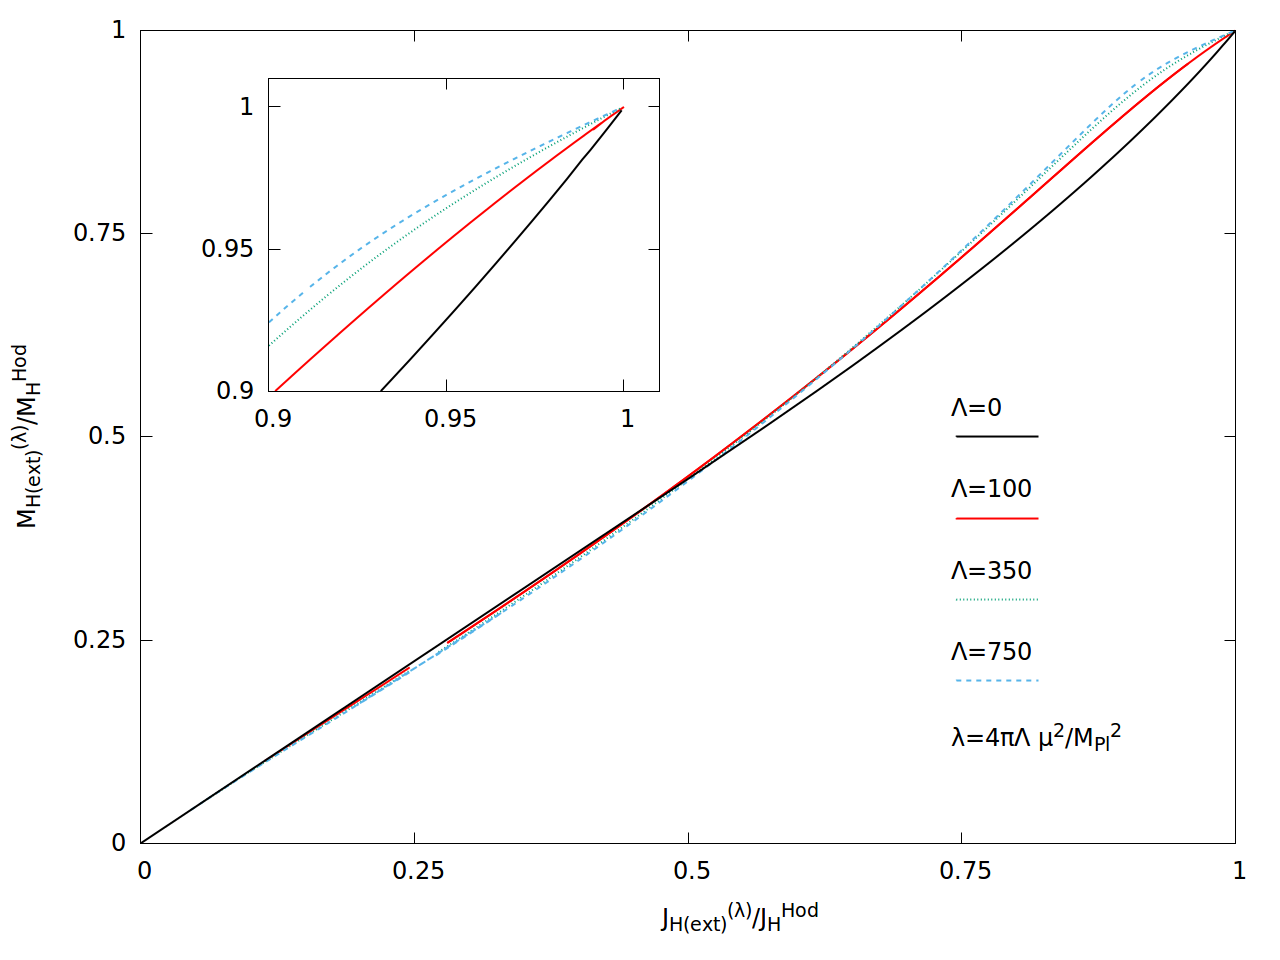
\includegraphics[width=0.7\textwidth]{papers/selfInteractions/horizon-ratios.png}
      \end{center}
      \caption{ The horizon quantities of extremal  KBHsSH and quartic-KBHsSH given in terms of the values at the Hod point, for different values of $\lambda$.}
  \label{horizon_ratios}
\end{figure}

To summarize, as the (quartic-)KBHsSH are bounded by the extremal KBHsSH line and the vacuum Kerr BH line,  and since both of these curves have their maxima at the Hod point, 
we conclude that the maximal horizon quantities are obtained at the Hod point and all 
(quartic-)KBHsSH will have horizon quantities that are
lower than those at the Hod point.



%%%%%%%%%%%%%%%%%%%%%%%%%%%%%%%%%%%%%%%%%%%%%%%%%%%%%%%%%%%%%%%%%%%%%%%%%
\section{Discussion: universality and phenomenology}
\label{sec_V}
%%%%%%%%%%%%%%%%%%%%%%%%%%%%%%%%%%%%%%%%%%%%%%%%%%%%%%%%%%%%%%%%%%%%%%%%%%%%%%%
The main, and somehow unexpected, result in this chapter is the observation that quartic-self interactions make KBHsSH ``hairier" but not ``heavier", in the sense of being able to increase their ADM mass but not their horizon mass, with respect to the maximal values attained in the absence of self-interactions. An immediate question is how \textit{universal} is this behaviour, if one considers a generic self-interacting scalar field theory.

To test this universality, we briefly consider a family of potentials discussed in Chapter \ref{ch:Q}.
I.e. $Q$-balls.

On the one hand, a systematic study of the spinning solitons 
(including the effects induced by the backreaction on the spacetime geometry) 
is given in \cite{Kleihaus:2005me}.
%As shown in Figure ??,
The results therein show that the
 generic gravitating boson stars in this theory, which we dub \textit{Q}-boson stars, follow closely the pattern for mini-boson stars and quartic-boson stars described herein; in particular 
one finds a similar, albeit somewhat distorted, version of the mass $vs.$ frequency diagram shown in Fig.~\ref{fig:w-vs-M-BSs}.

We have done some preliminary studies of backreacting $Q$-balls, and found families of KBHsSH with this type of self-interactions, which we dub $Q$-KBHsSH. The overall properties of these BH solutions are similar to those found herein for  quartic-KBHSSH.
In particular, the domain of existence is still bounded by the (corresponding)
curves ${\bf i)}$, ${\bf ii)}$ and ${\bf iii)}$ as defined in Section \ref{sec_III}. 
Therefore, the maximal ADM mass 
of the solutions is 
that of the corresponding $Q$-boson stars.
We remark that for the same scalar field mass, $Q$-KBHsSSH seem able to become considerably hairier than KBHsSH or quartic-KBHsSH.
%
An example of the domain of existence of $Q$-KBHsSH is presented in Fig.~\ref{qkbhsh} for a particular choice of couplings.
%
\begin{figure}[h!]
  \begin{center}
     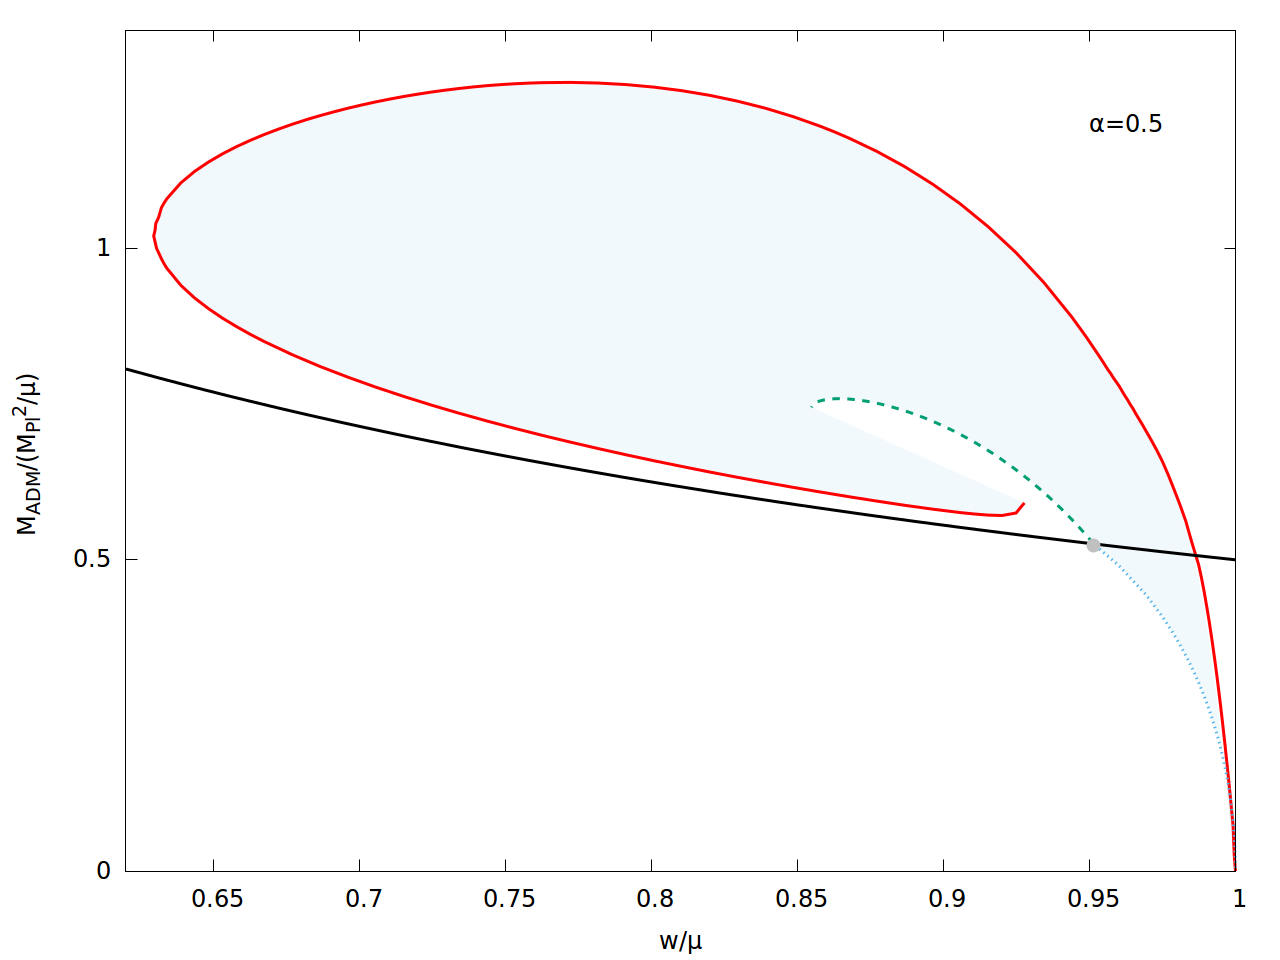
\includegraphics[width=0.7\textwidth]{papers/selfInteractions/w-vs-M-Q-a=05.png}
      \end{center}
  \caption{Domain of existence of a typical set of $Q$-KBHsSH (blue shaded region).}
  \label{qkbhsh}
\end{figure}
%


Concerning the horizon quantities, we have found
%the sextic-KBHsSSH do not become heavier.
that for all families of solutions studied so far,
 the pattern in 
Figs. \ref{horizon_phase} and \ref{horizon_ratios},   
is preserved.
In particular, the maximum of the horizon mass and angular momentum
are those of the (universal) Hod point - Fig.~\ref{horizon_ratios_q}

\begin{figure}[h!]
  \begin{center}
    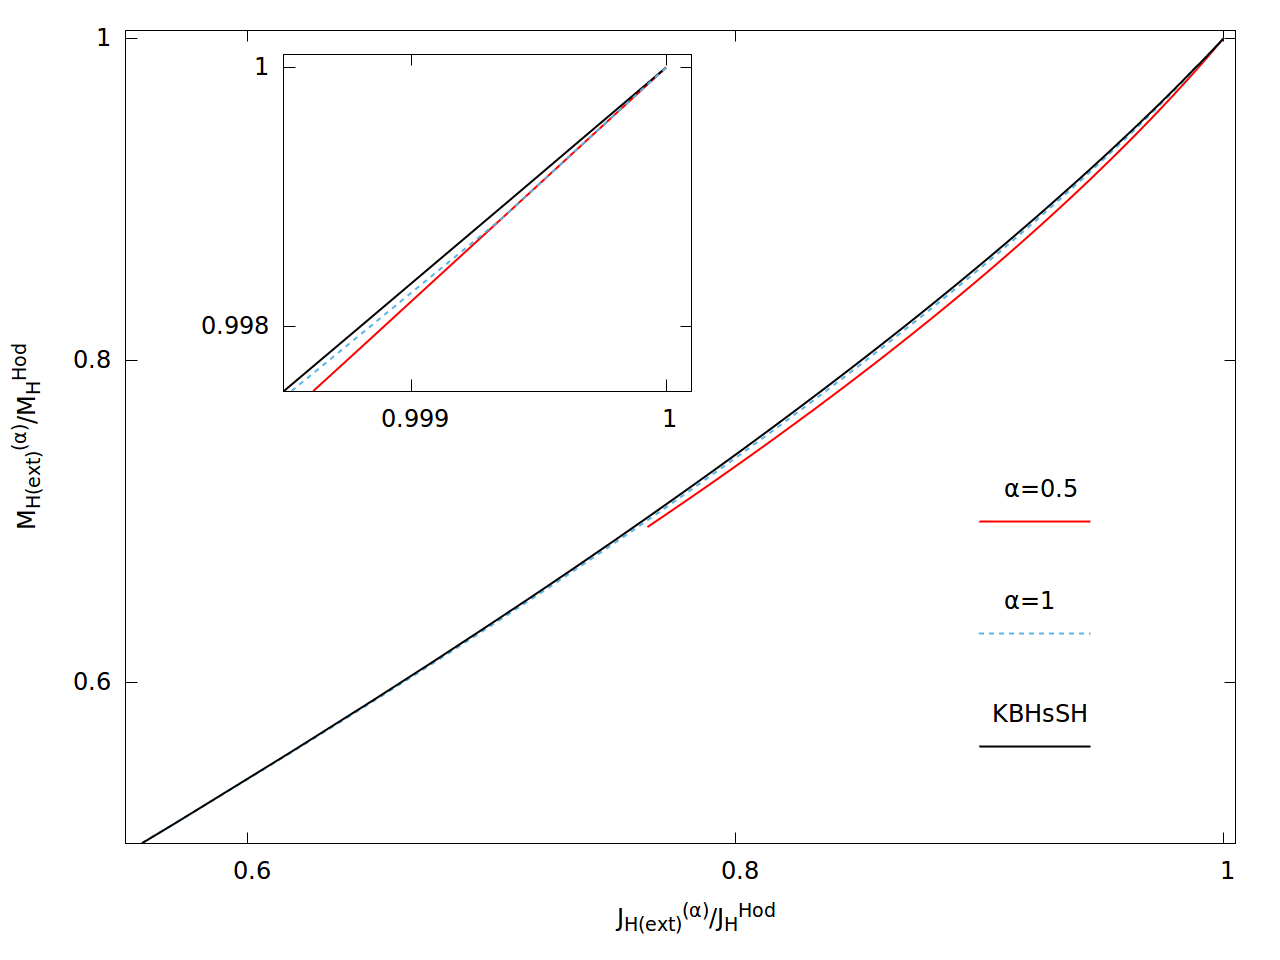
\includegraphics[width=0.7\textwidth]{papers/selfInteractions/horizon-ratios-Q.png}
      \end{center}
      \caption{ The horizon quantities of extremal  $Q$-KBHsSH given in terms of the values at the Hod point, for two different values of $\alpha$. The corresponding curve for KBHsSH without self-interactions almost overlaps with the $\alpha=1$ curve, confirming the behaviour described in the text.}
  \label{horizon_ratios_q}
\end{figure}


A final observation concerning $Q$-KBHsSH, that follows from our numerical data 
%exhibited by the sextic-KBHsSSH 
is that 
when increasing the coupling
constant  $\alpha$,
%the self-interaction terms become  irelavant  with increasing $\alpha$, 
the solutions tend to those with a free scalar field in \cite{Herdeiro:2014goa}. 
In fact, 
following the arguments in \cite{Kleihaus:2005me}, one can show that 
for large values of $\alpha$, all higher order terms in the scalar field potential become irrelevant
and, as $\alpha\to \infty$, one recovers the solutions of a model with a complex scalar field  
possessing a quadratic potential only. In fact, this feature starts to manifest already for $\alpha$  of order 1. This provides further evidence for the universality of the ``hairier" but not ``heavier" behaviour.

The result of this chapter is the following: the maximum horizon mass $M^{\rm max}_H$ for KBHsSH (with or without self-interactions) is attained at a particular configuration we dub the \textit{Hod point}, corresponding to the extremal (vacuum) Kerr BH obtained in the vanishing hair limit, and precisely one of the points studied in~\cite{Hod:2012px}.
For KBHsSH this maximal mass obeys the same form as \eqref{mini},
\begin{equation}
  M_{\rm H}^{\rm max}\simeq \alpha_{\rm Hod} \frac{M_{\rm Pl}^2}{\mu}\simeq \alpha_{\rm Hod} \, 10^{-19}M_\odot\left(\frac{\rm GeV}{\mu}\right)\ , 
\label{hodpoint}
\end{equation}
 but with the constant $\alpha_{\rm Hod}<\alpha_{\rm BS}$. For instance, for $m=1;2$, $\alpha_{\rm Hod}=0.526; 1.165$. 

\bigskip

Since the maximal horizon mass behaves as in Eq. \eqref{hodpoint}, if the ``hairier" but not ``heavier" property is universal and holds regardless of the scalar field theory, then KBHsSH with a trapped region with astrophysical masses can only exist if ultra-light scalars occur in Nature. This type of hairy BHs would be, therefore, a distinct observational signature of such beyond the Standard Model particles.
%
%
%
% \vspace{0.5cm} 
%  %%%%%%%%%%%%%%%%%%%%%%%%%%%%%%%%%%%%%%%%%%%%%%%%%%%%%%%%%%%%%%%%%%%
% \noindent
% \section*{Acknowledgements}
% C. H. and E. R. acknowledge funding from the FCT-IF programme. H.R. is supported by the grant PD/BD/109532/2015 under the MAP-Fis Ph.D. programme. This work was partially supported by the NRHEPÐ295189
% FP7-PEOPLE-2011-IRSES Grant, by FCT via project No.
% PTDC/FIS/116625/2010 and by the CIDMA strategic project UID/MAT/04106/2013. Computations were performed at the Blafis cluster, in Aveiro University.
%  
